\documentclass[11pt]{article}
\usepackage{graphicx}
\usepackage{amssymb}
\usepackage{bm}
\usepackage{mathtools}
\usepackage{amsmath}
\usepackage{commath}
\usepackage{amsthm}
\usepackage{enumitem}
\usepackage{float} 
\usepackage{array}
\usepackage{outlines}
\usepackage{setspace}
\usepackage[colorinlistoftodos]{todonotes}
\setlist[enumerate,1]{label=\alph*)}
\setlist[enumerate,2]{label=\roman*)}
\newtheorem{theorem}{Theorem}
\newtheorem{corollary}{Corollary}
\newtheorem{lemma}{Lemma}
\newtheorem{remark}{Remark}
\newtheorem{definition}{Definition}
\newtheorem{prop}{Proposition}
\newcommand*\diff{\mathop{}\!\mathrm{d}}
\usepackage{tikz}
\usetikzlibrary{arrows,shapes,trees, calc}

%%% some of the changes
%%% introduction of c = (c_h, c_3) Coriolis term in the equation for better readability in the estimate parts
%%% the Earth rotation vector is noted now by omega, instead of w // the u,v letters are associated with fluid velocity here, and omega is probably a more classical choice anyway
%%% to have a consistent horizontal component notation, let's choose u_h, with a small h. Let's use H letter only for Sobolev spaces
%%% in the estimates part let's use \partial_3 instead of \partial_z etc since at that point we are after the rescaling process

%%% *** PREAMBLE *** %%%
\title{A weak convergence result for the mathematical equations of the polluted atmosphere expressed in downwind matching coordinates}

\date{}

%%%***  CONTENT *** %%%
\begin{document}

\maketitle

\begin{abstract}

A widely used approach to mathematically describe the atmosphere is to consider it as a geophysical fluid in a shallow domain --- and thus to model it using classical fluid dynamical equations combined with the explicit inclusion of an $\epsilon$ parameter representing the small aspect ratio of the physical domain. In our previous paper \cite{pollatmws2019} we proved a weak convergence theorem for the polluted atmosphere described by the Navier-Stokes equations extended by an advection-diffusion equation. We obtained a justification of the generalised hydrostatic limit model including the pollution effect described in the case of a classical, east-north-upwards oriented local Cartesian coordinates. Here we give an improvement of this statement: we consider a meteorologically more meaningful coordinate system, incorporate the analytical consequences of this coordinate change into the governing equations, and verify that the weak convergence still holds for this altered concentration -- velocity system.

\end{abstract}

{\bf Keywords:} downwind-matching coordinate system, Navier-Stokes equations, shallow domains, pollution evolution equation, hydrostatic approximation, compactness, weak solutions.

\newpage

\tableofcontents
\newpage

%%% *** INTRODUCTION *** %%%
\section{Introduction} \label{Introduction}

A local domain on the surface of the rotating Earth is often described by a Cartesian coordinate system where the $x, y, z$ axes represent the directions towards east, north, and upwards, respectively, as in this specific system the rotation vector, and as a consequence, the Coriolis force takes a simpler form. However, for modelling wind and pollution effects in the atmosphere there is another naturally distinctive viewpoint for fixing the orientation of the coordinate system: the introduction of downwind and crosswind, and to match the horizontal axes according to these meteorological parameters (see \cite{goyal2011mathematical}). We take this idea as a foundation, and we migrate the result of our previously stated weak convergence theorem to this more considerately chosen coordinate system.

%% Here \todo{write this part} talk a little bit about the original convergence theorem to make the new one more self-contained and for details refer to the first article.

As in this scenario the advection is dominant compared to diffusion effects along the $x$ axis, this approach naturally contributes to an additional $\epsilon$ term in the Laplacian of the concentration equation, the simplification of the limit model, and brings the challenge of proving a weak convergence result for the product of the vertical velocity and the concentration, as in the energy inequality the $\norm{\partial_1 C^\epsilon}$ term is replaced by $\norm{\sqrt{\epsilon} \partial_1 C^\epsilon}.$ This issue is overcome by using a more regular initial horizontal velocity function, namely $\mathbf{v} \in H^1.$ The additional, stronger initial regularity will result in a smoother $\mathbf{u}^\epsilon$ function, and thus will make up for the lost $H^1$ regularity of the concentration function $C.$

We will also use slightly different, stricter boundary conditions --- these additional requirements are motivated by \textit{a)} the presence of $\epsilon$ next to the sediment functions, and \textit{b)} the need to eliminate certain boundary terms in the new part of the proof, which is based on a result obtained for a periodic domain (\cite{li2019primitive}).

We end up this section with some notations we will use through the paper.

\subsection{Notations}

\begin{enumerate}

\item $\epsilon = $ the aspect ratio,
\item $\nu = $ viscosity,
\item $\Omega_\epsilon, \Omega = $ the original and the rescaled ($\epsilon$-independent) domain, respectively,
\item $\nabla$ stands for the gradient vector; specifically, $(\partial_x, \partial_y, \partial_z)$ before, and $(\partial_1, \partial_2, \partial_3)$ after rescaling,
\item $\nabla_\nu = (\nu_x^{1/2} \partial_x, \nu_y^{1/2} \partial_y, \nu_z^{1/2} \partial_z)$ on $\Omega_\epsilon$, $\nabla_\nu = (\nu_1^{1/2} \partial_1, \nu_2^{1/2} \partial_2, \nu_3^{1/2} \partial_3)$ on the rescaled domain $\Omega,$
\item $ \Delta_\nu$ stands for the anisotropic Laplacian operators $\nu_x \partial^2_{xx} + \nu_y \partial^2_{yy}  + \nu_z \partial^2_{zz}$ and $\nu_1 \partial^2_{11} + \nu_2 \partial^2_{22}  + \nu_3 \partial^2_{33}$ on the original and rescaled domains, respectively,
\item $\mathbf{g}$ represents the force due to gravity, which also includes the centrifugal effect,
\item $\varphi = $ the gravity potential term, i.e. $\mathbf{g} = \nabla \varphi,$
\item $\mathbf{\omega}$ represents the Earth rotation angular speed,
\item $\phi = l(y) = $ latitude, $f = $ the module of the Earth rotation vector
\item $\alpha = -2 f \sin(\theta)\cos(\phi), \beta = 2 f \cos(\theta) \cos(\phi), \gamma = 2 f \sin(\phi),$
\item $\mathbf{c}(\mathbf{u}) = (\mathbf{c}_h (\mathbf{u}), c_3 (\mathbf{u}_h)) = ( -\gamma u_2^\epsilon + \epsilon \beta u_3^\epsilon, \alpha \epsilon u^\epsilon_3 - \gamma u_1^\epsilon, \alpha u^\epsilon_2 - \beta u_1^\epsilon),$ the Coriolis force terms 
\item $\mathbf{K}$ represents the diagonal diffusion matrix,
\item $( \cdot,\cdot) = $ the scalar product in $L^2(\Omega)^d$ or the duality $L^p (\Omega)$, $L^{p'} (\Omega),$
\item $< \cdot,\cdot>_{\Gamma} = $ the scalar product or duality on the boundary curve $\Gamma$ ($H^{-1/2}(\Gamma)$, $H^{1/2}(\Gamma)$),
\item $\mathbf{u}_h$ = the horizontal velocity components $(u_1, u_2),$
\item $b(\mathbf{u}_h)$ = $- \gamma (u_2 , u_1),$
\item $L^p_t L^q_x$ is the abbreviated notation for $L^p (0, T; L^q(\Omega)).$

\end{enumerate}

%%% *** THE POLLUTED ATMOSPHERE MODEL *** %%%
\section{The polluted atmosphere model} \label{eqsdescribingatmpluspollution}

As we highlighted before, the key point of this new model is to integrate some of the main ideas of a Gaussian plume dispersion model into the system describing the polluted atmosphere. Therefore we begin by fixing the local Cartesian coordinate system to be adjusted to the downwind direction, i.e. $z$ is oriented upwards, while $x$ is the downwind, and $y$ is the crosswind direction. Another assumption the Gaussian dispersion models typically use as well is that advection is more dominant than diffusion along the downwind direction, which leads to the appearance of an additional $\epsilon$ term in the concentration equation's Laplacian. Namely, we have

\begin{equation} \abs{u_1 \partial_{1} C} \gg \abs{ K_x \partial_{11} ^2 C }\end{equation}

which leads us to using this additional scaling equation

\begin{equation} \label{ksepsk1} K_x = \epsilon K_1.\end{equation}

\begin{remark} \normalfont
  The inclusion of these two features in a pollution model are legitimate when the following circumstances hold:
  \begin{itemize}
    \item We are considering a time interval which is not too long in the sense that it is reasonable to assume that we have a permanent, relatively stable main wind direction, i.e. fixing the horizontal coordinates is reasonable in the first place,
    \item There is an adequate, relatively high wind speed --- low wind speeds in general lead to a situation where three dimensional diffusion dominates, leading to an error caused by the dominant advection assumption. Fast changing wind direction and low windspeed resulting in fast pollutant settling can make it extremely challenging to obtain reliable results from Gaussian models.
  \end{itemize}
\end{remark}

Choosing the coordinate system in this particular way results in changes in three main points of the system. One of these is the Coriolis term, since now the $x$ axis is not necessarily perpendicular to the rotation vector. We need to revisit the boundary conditions as well, and as discussed above, a modification in the pollution concentration equation also has to be taken into account. We will describe these changes and their consequences in detail --- the main challenge in proving this paper's convergence result is in fact to handle the effect of this latter change on the energy inequality.

In order to obtain the set of equations that describe the phenomena we start with the original set of equations

\begin{equation} \label{originalEQ-V}
  \partial_t \mathbf{v} + (\mathbf{v} \cdot \nabla)\mathbf{v} -\Delta_{\nu} \mathbf{v} + \nabla q + 2 \mathbf{\omega} \times \mathbf{v}= \mathbf{g} \text{ in } \Omega_{\epsilon} \times (0,T)
\end{equation}
    
\begin{equation} \label{originalEQ-I}
  \nabla \cdot \mathbf{v} = 0 \text{ in } \Omega_{\epsilon} \times (0,T)
\end{equation}
    
\begin{equation} \label{diffusive}
  \partial_t P + \mathbf{v} \cdot \nabla P = \nabla \cdot (\mathbf{K} \nabla P) + Q,
\end{equation}

As for the rescaling process, here we perform the same steps, with the addition of $(\ref{ksepsk1}).$

To expand the $2 \mathbf{\omega} \times \mathbf{v}$ Coriolis term, firstly it is necessary to understand the structure of the new rotation vector. Note that the downwind-matching coordinate system and the original east-north-upwards oriented system are different only in a rotation around the $z$ axis. Let $\theta$ denote the angle between the respective $x$ axes, $\phi$ denotes the latitude, then the rotation vector expressed in the downwind matching coordinate system becomes

\begin{gather}
 \begin{bmatrix} \cos(\theta) & -\sin(\theta) & 0 \\ \sin(\theta) & \cos(\theta) & 0 \\ 0 & 0 & 1 \end{bmatrix} \begin{bmatrix} 0 \\ f \cos(\phi) \\ f \sin(\phi) \end{bmatrix}
 =
  f \begin{bmatrix} -\sin(\theta)\cos(\phi) \\ \cos(\theta) \cos(\phi) \\ \sin(\phi) \end{bmatrix}.
\end{gather}

Now, let

$$\alpha = -2 f \sin(\theta)\cos(\phi), \quad \beta = 2 f \cos(\theta) \cos(\phi), \quad \gamma = 2 f \sin(\phi),$$

and using this, the Coriolis force takes the form

\begin{gather}
\begin{bmatrix} \alpha \\ \beta \\ \gamma \end{bmatrix}
 \times
 \begin{bmatrix} u_1 \\ u_2 \\ \epsilon u_3 \end{bmatrix}
 =
 \begin{bmatrix}  \beta \epsilon u_3 - \gamma u_2 \\ \gamma u_1 - \alpha \epsilon u_3  \\ \alpha u_2 - \beta u_1 \end{bmatrix}.
\end{gather}

Thus, these are the terms that appear in the three velocity equations; and finally, note that the third component is present in the rescaled version of the vertical velocity equation multiplied by $\epsilon,$ which is obtained from the $\epsilon$ term in the denominator of $\partial_z p.$

\begin{remark} \normalfont
The intuitive meaning of what we understand by downwind and the velocity in this new coordinate system: the downwind direction is an approximately steady-in-time direction, it can be seen as the direction marked by the wind direction trackers on an airport or meteorological point. When we consider the downwind, we neglect the small perturbations in its orientation, it can be viewed as a time-averaged direction as long as the fluctuation is relatively small. On the other hand, the velocity is a three dimensional, time dependent vector that changes second after second. 

\end{remark}
    
    We arrive to the merged anisotropic equations of the polluted atmosphere above inland surface:
  
    \begin{equation} \label{ANSC1}
    \partial_t u^\epsilon _1 + \mathbf{u}^\epsilon \cdot \nabla u^\epsilon _1 -\Delta_\nu u^\epsilon _1 -\gamma u_2^\epsilon + \epsilon \beta u_3^\epsilon + \partial_1 p^\epsilon = 0 \text{ in } \Omega \times (0,T)
    \end{equation}
    
    \begin{equation} \label{ANSC2}
    \partial_t u_2^\epsilon + \mathbf{u}^\epsilon \cdot \nabla u_2^\epsilon -\Delta_\nu u_2^\epsilon + \gamma u_1^\epsilon - \alpha \epsilon u^\epsilon_3  + \partial_2 p^\epsilon = 0 \text{ in } \Omega \times (0,T)
    \end{equation}
    
    \begin{equation} \label{ANSC3}
    \epsilon^2 \{  \partial_t u_3^\epsilon + \mathbf{u}^\epsilon \cdot \nabla u_3^\epsilon -\Delta_\nu u_3^{\epsilon} \} + \epsilon \alpha u^\epsilon_2 - \epsilon \beta u_1^\epsilon + \partial_3 p^\epsilon = 0 \text{ in } \Omega \times (0,T)
    \end{equation}
    
    \begin{equation} \label{ANSC4}
    \nabla \cdot \mathbf{u}^\epsilon= 0 \text{ in } \Omega \times (0,T)
    \end{equation}
    
    \begin{equation} \label{ANSC5}
    \partial_t C^\epsilon + \mathbf{u^\epsilon} \cdot \nabla C^\epsilon = \epsilon K_1 \partial_{11} ^ 2 C^\epsilon + K_2 \partial_{22} ^ 2 C^\epsilon + K_3 \partial_{33} ^ 2 C^\epsilon + S_\epsilon \text{ in } \Omega \times (0,T)
    \end{equation}

The initial condition for the velocity and the pollution concentration are
    
    \begin{equation} \label{ANSC7}
    \mathbf{u}^\epsilon (\cdot, t = 0) = \mathbf{u}_0, \quad C^\epsilon (\cdot, t=0) = C_0  \quad \text{ in } \Omega.
    \end{equation}
  
  Finally, the boundary conditions to describe the anisotropic system can be summarised as follows:
  
    \begin{equation} \label{ANSC8}
      \begin{split}
        & \mathbf{u}^\epsilon = 0 \text{ on } \Gamma \times (0,T), \\
        &C^\epsilon = 0 \text{ on } ( \Gamma_U \cup \Gamma_L) \times (0,T), \\
        & \partial_2 C^\epsilon = \partial_3 C^\epsilon = 0 \text{ on } \Gamma_G \times (0,T), \quad \partial_1 C^\epsilon \in L^2 L^2 (0,T; \Gamma_G), \\
      \end{split}
    \end{equation}
    
    where the boundary structure of the domain is identical to what we used in \cite{pollatmws2019}, i.e. the upper boundary of the $\Omega$ domain is denoted by $\Gamma_U$, the lateral boundary is $\Gamma_L$, and the lower boundary of the domain is $\Gamma_G$, while the complete boundary is denoted by $\Gamma$ (see graph later.)
    
    \begin{figure}[!h]
  \centering
  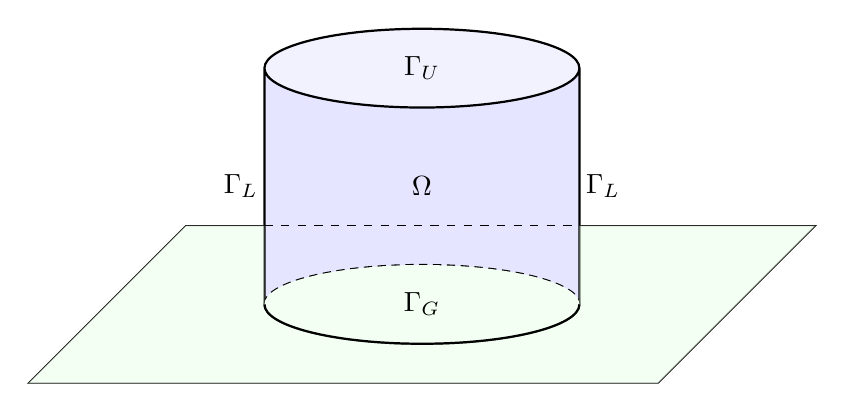
\begin{tikzpicture}
    \fill[color=blue!10] (2,0) -- (2,3) arc (360:180:2cm and 0.5cm) -- (-2,0) arc (180:360:2cm and 0.5cm);
    \fill[color=blue!5] (0,3) circle (2cm and 0.5cm);
    
    \draw[thick] (-2,3) -- (-2,0) arc (180:360:2cm and 0.5cm) -- (2,3) ++ (-2,0) circle (2cm and 0.5cm);
    \draw[densely dashed, thick] (-2,0) arc (180:0:2cm and 0.5cm);
    \draw (-2,1) -- (-3,1) --(-5,-1) -- (3,-1) -- (5,1) -- (2,1);
    \draw[dashed] (-2,1) -- (2,1);
    
    \fill[green!10,opacity=0.5] (-2,0) -- (-2,1) -- (-3,1) -- (-5,-1) -- (3,-1) -- (5,1) -- (2,1) -- (2,0) arc (0:180:2cm and -0.5cm);
    \fill[color=green!5] (0,0) circle (2cm and 0.5cm);
    
    \draw (0,1.5) node {$\Omega$};
    \draw (0,3) node {$\Gamma_U$};
    \draw (0,0) node {$\Gamma_G$};
    \draw (-2.3,1.5) node {$\Gamma_L$};
    \draw (2.3,1.5) node {$\Gamma_L$};
    
    \draw[thick] (2,0) arc (360:180:2cm and 0.5cm);
  \end{tikzpicture}
\end{figure}
    
We highlight the difference between the boundary conditions of the original, east-north oriented, and the new, downwind-matching model.

The difference in the kind of boundary conditions that we can "afford" to have on the lower boundary for the concentration comes from the energy inequality. In the east-north-upwards oriented coordinate system we do not have an $\epsilon$ in the diffusion matrix, and thus it is not an issue to have any of the $\partial_i C$ terms to be different from 0, not even for an ocean case where $\partial_3 C$ becomes nonzero as well (they are required however to be bounded of course). On the other hand, the downwind-matching coordinate system brings in an $\epsilon$ term in front of the $K_1$ diffusion, which makes the model more sensitive to assigning boundary conditions for $C.$ This means that we can not have the relatively relaxed, boundedness requirement for any $\partial_i C$ except for $i=1.$ All other $\partial_2 C, \partial_3 C$ derivatives must be zero on the lower boundary, otherwise they would result in an $(\epsilon - \text{const.})$ negative term --- for more details see the energy inequality of the system in the section describing the proof. This also means that we will consider exclusively the inland domain scenario.

If we assume $\mathbf{u}^\epsilon = O(1)$, then neglecting the $\epsilon^2$ and $\epsilon$ in the anisotropic equations, we formally arrive to the hydrostatic Navier-Stokes equations (i.e., primitive equations) combined with pollution.

    \begin{equation} \label{HNSC1}    
    \partial_t u_1 + \mathbf{u} \cdot \nabla u_1 - \Delta_\nu u_1 -\gamma u_2 + \partial_1 p = 0 \text{ in } \Omega \times (0,T)
    \end{equation}
    
    \begin{equation} \label{HNSC2}   
    \partial_t u_2 + \mathbf{u} \cdot \nabla u_2 - \Delta_\nu u_2 + \gamma u_1 + \partial_2 p = 0 \text{ in } \Omega \times (0,T)
    \end{equation}
    
    \begin{equation} \label{HNSC3}   
    \partial_3 p = 0 \text{ in } \Omega \times (0,T)
    \end{equation}
    
    \begin{equation} \label{HNSC4}   
    \nabla \cdot \mathbf{u} = 0 \text{ in } \Omega \times (0,T)
    \end{equation}
    
    \begin{equation} \label{HNSC5}   
    \partial_t C + \mathbf{u} \cdot \nabla C = K_2 \partial_{22} ^ 2 C + K_3 \partial_{33} ^2 C + S \text{ in } \Omega \times (0,T)
    \end{equation}
    
    \begin{equation} \label{HNSC6}   
    u_1 = u_2 = u_3 = 0 \text{ on } \Gamma \times (0,T)
    \end{equation}
    
    \begin{equation} \label{HNSC7}   
    u_i (\cdot, t=0) = u_{0 i}, C (\cdot, t=0) = C_0 \text{ in } \Omega, \text{$i$ = 1,2}
    \end{equation}
    
    \begin{equation} \label{HNSC8}
      \begin{split}
        & C = 0 \text{ on } ( \Gamma_U \cup \Gamma_L) \times (0,T), \\
        & \partial_2 C = \partial_3 C = 0 \text{ on } \Gamma_G \times (0,T), \partial_1 C \in L^2 L^2 (0,T; \Gamma_G) \\
      \end{split}
    \end{equation}
    
    \begin{remark}
    \normalfont Note that in this case we have the more regular $v_0 \in H^1$ condition, so we will use the $u_3 = 0$ equality on the boundary directly, instead of the original $u_3 n_3 = 0$ constraint that we used.
    \end{remark}
    
    \begin{remark}
    \normalfont The $S^\epsilon$ and $S$ source terms are defined to be the nascent delta function with parameter $\epsilon$ and the delta distribution, respectively; both centred at $\mathbf{x_s}$, with an activation multiplier set to $t_s$. For more details see \cite{pollatmws2019}.
    \end{remark}

%%% *** WEAK FORMULATION AND MAIN RESULT*** %%%
\section{Weak Formulation and Main Result} \label{weakformulationmainresult}

In this section we describe the weak formulation of the merged equations in both the anisotropic and hydrostatic case, and we state our main result.
  
  We need to define the following spaces:
  
  \[ C^{\infty}_\Gamma (\Omega) = \{ \varphi \in C^\infty (\bar{\Omega}); \varphi = 0 \text{ on some neighbourhood of } \Gamma\} \]
  
  \[ H^k_{\Gamma} (\Omega) = \overline{C_\Gamma ^ \infty (\Omega)} ^ {H^k (\Omega)} = \{ v \in H^k(\Omega); v=0 \text{ on } \Gamma \} \]
  
  \[ \mathbf{V} = \{ \mathbf{v} \in  H^1_{\Gamma} (\Omega) \times H^1_{\Gamma} (\Omega) \times H^1_0 (\Omega); \nabla \cdot \mathbf{v} = 0 \text{ in } \Omega \} \]
  
  \[ H (\partial_3, \Omega) = \{ v \in L^2(\Omega); \partial_3 v \in L^2 (\Omega)\} \]
  
  \[ H_0 (\partial_3, \Omega) = \overline{C_0 ^\infty (\Omega)}^{H (\partial_3, \Omega)} = \{ v \in H(\partial_3, \Omega); v n_3 = 0 \text{ on } \Gamma \} \]
  
  \[ \mathbf{W} = \{ \mathbf{u} \in  H^1_{\Gamma} (\Omega) \times H^1_{\Gamma} (\Omega) \times H_0 (\partial_3, \Omega); \nabla \cdot \mathbf{u} = 0 \text{ in } \Omega \} \]
  
  Then the weak formulation of the hydrostatic system (\ref{HNSC1}) - (\ref{HNSC8}) takes the following form.
  
  \begin{definition} \label{definitionhydrostaticWF}
  
  Find $(\mathbf{u}, C)$ such that $\mathbf{u} = (\mathbf{u}_H, u_3) \in L^2 (0, T; \mathbf{W})$ with $\mathbf{u}_H \in L^\infty (0,T; L^2(\Omega)^2),$ and $C \in L_t^\infty L_x^2$ with $\partial_2 C, \partial_3 C \in L^2_t L^2_x$, such that
  
  \begin{equation}
    \begin{split}
      & \int_0^T \bigg[ -(\mathbf{u}_H, \partial_t \mathbf{\tilde{u}}_H) + (\nabla_\nu \mathbf{u}_H, \nabla_\nu \mathbf{\tilde{u}}_H) - (\mathbf{u}_H, (\mathbf{u} \cdot \nabla) \mathbf{\tilde{u}}_H) + (b(\mathbf{u}_H), \mathbf{\tilde{u}}_H) \bigg ] \diff t \\
      & = - (\mathbf{u}_{0H}, \mathbf{\tilde{u}}_H(0)) \diff t \label{hydrostaticWF}
    \end{split}
  \end{equation}
  
  and
  
  \begin{equation}
    \begin{split} \nonumber
      &+ \int_0^T \bigg[ -(C, \partial_t \tilde{C}) -(\mathbf{u}C, \nabla \tilde{C}) + K_2 (\partial_2 C, \partial_2 \tilde{C}) + K_3 (\partial_3 C, \partial_3 \tilde{C}) \bigg ] \diff t \\
      & = - (C(0), \tilde{C}(0)) + \int_0^T (S,\tilde{C}) \diff t
    \end{split}
  \end{equation}
  
  for all $(\mathbf{\tilde{u}}, \tilde{C})$ with $\mathbf{\tilde{u}} = (\mathbf{\tilde{u}}_H, \tilde{u}_3) \in H^1 (0,T, \mathbf{W})$, with $\mathbf{\tilde{u}}_H (T) = 0$ and $\partial_3 \mathbf{\tilde{u}}_H \in L^\infty (0, T; L^3 (\Omega)^2)$ and $\tilde{C}$ with $\tilde{C} \in L^2 (0,T, H^3_{\Gamma} (\Omega))$, $\tilde{C} \in H^1 (0,T, L^2)$, $\tilde{C} (T) = 0$. 
  
  \end{definition}
  
  Giving definition to the weak formulation of the anisotropic system we underline the importance of the spaces we use here --- they create a sort of in-between point between classical weak solutions and Leray-Hopf weak solutions in the sense that the concentration function does not need to be weakly continuous, but the velocity part of the solution is set to be in $C_w.$ This represents a space construction that is both minimal and corresponds to the requirements of the proof detailed later.

 \begin{definition} \label{definitionanisotropicWF}
  
  Find $\mathbf{u}^\epsilon = (\mathbf{u}_H, u^\epsilon_3) \in L^2 (0,T ; \mathbf{V}) \cap C_w (0, T; L^2 (\Omega)^3)$ and $C^\epsilon \in L^\infty (0,T; L^2(\Omega)) \cap L^2 (0,T; H^1(\Omega))$, such that
  
  \begin{equation}
    \begin{split}
      & \int_0^T \bigg [ -(\mathbf{u}^\epsilon_H, \partial_t \mathbf{\tilde{u}}_H) + (\nabla_\nu \mathbf{u}^\epsilon_H, \nabla_\nu \mathbf{\tilde{u}}_H) - (\mathbf{u}^\epsilon_H, (\mathbf{u}^\epsilon \cdot \nabla) \mathbf{\tilde{u}}_H) + (b(\mathbf{u}^\epsilon_H), \mathbf{\tilde{u}}_H) \bigg ] \diff t \\
      & + \epsilon \beta \int_0 ^ T \big [ (u_3 ^\epsilon, \tilde{u}_1) - (u_1^\epsilon, \tilde{u}_3) \big ] \diff t\\
      & + \epsilon^2 \int _0 ^ T \big [ -(u_3^\epsilon, \partial_t \tilde{u}_3) +(\mathbf{u}^\epsilon \cdot \nabla u_3 ^ \epsilon, \tilde{u}_3) + (\nabla_\nu u_3^\epsilon, \nabla_\nu \tilde{u}_3) \big ] \diff t \\
      & = - (\mathbf{u}^\epsilon_{0H}, \mathbf{\tilde{u}}_H(0)) - \epsilon^2 (u_{03}^\epsilon, \tilde{u}_3 (0)) \diff t \raisetag{20pt} \label{anisotropicWF}
    \end{split}
  \end{equation}
  
    and
  
    \begin{equation}
    \begin{split} \nonumber
      & \int_0^T \bigg [ -(C^\epsilon, \partial_t \tilde{C}) -(\mathbf{u}^\epsilon C^\epsilon, \nabla \tilde{C}) + \epsilon K_1 (\partial_1 C^\epsilon, \partial_1 \tilde{C}) - \epsilon K_1 \big[(\partial_1 C^\epsilon) \tilde{C} \big] _{\Gamma_G} \\
      & + K_2 (\partial_2 C^\epsilon, \partial_2 \tilde{C}) + K_3 (\partial_3 C^\epsilon, \partial_3 \tilde{C}) \bigg ] \diff t \\
      & =  - (C^\epsilon (0), \tilde{C} (0)) + \int_0^T (S^\epsilon,\tilde{C}) \diff t
    \end{split}
  \end{equation}
  
  for all $\mathbf{\tilde{u}} = (\mathbf{\tilde{u}}_H, \tilde{u}_3) \in H^1 (0,T;\mathbf{V})$ with $\mathbf{\tilde{u}}(T) = 0$ and $\tilde{C}$ such that $\tilde{C} \in H^1 (0,T, H^3_{\Gamma} (\Omega))$ and $\tilde{C} (T) = 0$.
  
  \end{definition}

The main theorem of this paper is analogous to our previous result stated for the case of the geophysical frame, but we highlight the difference that here we use the initial data $\mathbf{v}_0 \in H^1.$ For the case of the geophysical frame an $L^2$ initial velocity was sufficient, here we need a stronger data to balance out the weaker results we can extract from the energy inequality on $C^\epsilon.$

Now we are ready to state the main theorem.

\begin{theorem} \label{maintheorem}
  Let $\mathbf{v}_0$ $\in$ $H^1 (\Omega)$, ${u_3}_0 \in L^2(\Omega)$ with $\nabla \cdot \mathbf{u}_0 = 0, \mathbf{u}_0 \cdot \mathbf{n} = 0$ on $\partial \Omega$; let $C_0 \in$ $L^2 (\Omega)$, $C_0 = 0$ on $ \partial \Omega$, and assume that the boundary conditions (\ref{ANSC8}) hold; then as the aspect ratio $\epsilon$ tends to zero, any weak solution $(\mathbf{u}^\epsilon, C^\epsilon)$ of the anisotropic equations (\ref{ANSC1}) - (\ref{ANSC5}) converges to a weak solution $(\mathbf{u}, C)$ of the hydrostatic equations of the polluted atmosphere (\ref{HNSC1}) - (\ref{HNSC5}).
\end{theorem}
  
%%% *** PROOF *** %%%

\section{Proof of the main theorem} \label{proof}

This section is devoted to verify Theorem \ref{maintheorem}. Structurally we follow a similar chain of thought as in our previous paper --- until the point where the proof diverges reaching the weak convergence of the nonlinear term $u_3^\epsilon C^\epsilon$ where in this case we can not benefit from an $H^1$ regular concentration function. In more detail, we begin with calculating the energy inequality and collect the a priori estimates that derive from it, then verify the rather easily obtainable weak convergence results. Finally we elaborate the steps to bring to a closure the convergence of the $u_3^\epsilon C^\epsilon$ term. The main idea here is to temporarily ignore the $C^\epsilon$ function and prove a strong convergence result considering only the velocity functions. Throughout this step we go beyond the weak solutions quality and show that we are working with strong solutions. In this new setting with more favorable regularities we can prove the convergence result we need, and eventually return to the frame of weak solutions where we can merge back together the velocity and concentration functions into a unified solution.

  \subsection{Energy inequality}
  
  Calculating the energy inequality for the anisotropic system, we obtain that for a.e. $t \in [0,T]$ the following holds:
  
  \begin{equation}
    \begin{split}  
    & \frac{1}{2} (\norm{\mathbf{u}_H^\epsilon (t)}_{L^2}^2 + \epsilon ^ 2 \norm{u_3^\epsilon (t)}_{L^2}^2 + \norm{C^\epsilon (t)}_{L^2}^2) + \int_0 ^ t \big[ \norm{\nabla_\nu \mathbf{u}_H^\epsilon}_{L^2}^2 + \epsilon ^ 2 \norm{\nabla_\nu u_3^\epsilon}_{L^2}^2  \big] \diff \tau \\
    & + \int_0 ^ t  \big [ \epsilon K_1 \norm{\partial_1 C^\epsilon}_{L^2}^2  + K_2 \norm{\partial_2 C^\epsilon}_{L^2}^2 + K_3 \norm{\partial_3 C^\epsilon}_{L^2}^2 \big ] d \tau \\
    & \leq \int_0^t (S^\epsilon,C^\epsilon) \diff \tau + \frac{1}{2} (\norm{\mathbf{u}_H^\epsilon (0)}_{L^2}^2 + \epsilon ^ 2 \norm{u_3^\epsilon (0)}_{L^2}^2 + \norm{C^\epsilon_0}_{L^2}^2) \\
    & + \int _ 0 ^ t \epsilon K_1 \langle \partial_1 C^\epsilon, C^\epsilon \rangle_{\Gamma_G} \diff \tau \raisetag{70pt} \label{energyIEQ}
    \end{split}
  \end{equation}
  
  Using standard techniques, the generalised Young inequality with a $\zeta > 0$ constant, the Holder inequality and the Trace Theorem, (\ref{energyIEQ}) takes the final form

  \begin{equation}
    \begin{split}  
    & \frac{1}{2} (\norm{\mathbf{u}_H^\epsilon (t)}_{L^2}^2 + \epsilon ^ 2 \norm{u_3^\epsilon (t)}_{L^2}^2 + \norm{C^\epsilon (t)}_{L^2}^2) + \int_0 ^ t \big [\norm{\nabla_\nu \mathbf{u}_H^\epsilon}_{L^2}^2 + \epsilon ^ 2 \norm{\nabla_\nu u_3^\epsilon}_{L^2}^2 \big ] \diff \tau \\
    & + \int_0 ^ t \bigg[ (\epsilon K_1 - \zeta \frac{\epsilon}{2} K_1 c_T (c_S + 1)) \norm{\partial_1 C^\epsilon}_{L^2}^2  + (K_2 - \zeta \frac{\epsilon}{2} K_1 c_T (c_S + 1)) \norm{\partial_2 C^\epsilon}_{L^2}^2 \\
    & + (K_3 - \zeta \frac{\epsilon}{2} K_1 c_T (c_S + 1)) \norm{\partial_3 C^\epsilon}_{L^2}^2 \bigg] \diff \tau \\
    & \leq \frac{1}{\zeta} K_1 \frac{\epsilon}{2} \int_0 ^ t \norm{\partial_1 C^\epsilon}^2 _{L^2 (\Gamma_G)} + \frac{1}{2} (\norm{\mathbf{u}_H^\epsilon (0)}_{L^2}^2 + \epsilon ^ 2 \norm{u_3^\epsilon (0)}_{L^2}^2 + \norm{C^\epsilon (0)}_{L^2}^2) \\
    & + \int_0^t (S^\epsilon,C^\epsilon) \diff \tau, \raisetag{20pt} \label{finalformEIEQ}
    \end{split}
  \end{equation}
  
  where $c_T$ and $c_S$ are the constants provided by the Trace Theorem and Sobolev embeddings. The boundary term is bounded because of the a priori assumptions made on the boundary conditions.
    
  The right hand side of the energy inequality is now apparently bounded, and it is easy to see that the coefficients of the pollution terms are positive, since the $\zeta$ constant of the generalised Young inequality can be freely chosen in a way such that the requirements $\epsilon K_1 (1 - \zeta \frac{1}{2} c_T (c_S + 1)) > 0, (K_2 - \zeta \frac{\epsilon}{2} K_1 c_T (c_S + 1)) > 0, (K_3 - \zeta \frac{\epsilon}{2} K_1 c_T (c_S + 1)) > 0 $ are all satisfied.
  
  We note that he most significant difference in this new form of the energy inequality (\ref{finalformEIEQ}) is having $\sqrt{\epsilon} \partial_1 C^\epsilon$ in the place of $\partial_1 C^\epsilon,$ which is what we had for the case of the geophysical coordinate system. It leads to the disappearance of the $H^1$ regularity of $C^\epsilon,$ and thus we don't the strong convergence feature of the concentration function which was of key importance in the previous version for proving the weak convergence of a nonlinear term.
  
  This form of the energy inequality also shows why the $\partial_2 C^\epsilon, \partial_3 C^\epsilon$ terms need to vanish on the boundary. Otherwise, using the Trace Theorem on these boundary terms would contribute to the appearance of negative $\epsilon$-free terms in the coefficient of $\norm{\partial_1 C^\epsilon}_{L^2}^2,$ which would ruin the structure of the energy inequality.
  
  \subsection{A priori estimates. Weak convergence - Part 1.}
  
  From the final form of the energy inequality (\ref{finalformEIEQ})we obtain uniform a priori estimates that we summarise in the following proposition.
  
  \begin{prop} \label{aprioriprop}
    Let $u^\epsilon_1, u^\epsilon_2, u^\epsilon_3$ and $C^\epsilon$ be the weak solutions of the system (\ref{ANSC1}) - (\ref{ANSC5}) in the sense of Definition \ref{definitionanisotropicWF}. Then it holds,
    
    \begin{align}
      & u^\epsilon_1, u^\epsilon_2, \epsilon u^\epsilon_3, C^\epsilon & \quad & \text{are bounded in $L^\infty (0,T; L^2(\Omega)),$} \label{proposition1} \\
      & u^\epsilon_3 & \quad & \text{is bounded in $L^2 (0,T; L^2(\Omega)),$} \label{propositionExtra} \\
      & u^\epsilon_1, u^\epsilon_2, \epsilon u^\epsilon_3 & \quad & \text{are bounded in $L^2(0,T; H^1(\Omega)),$} \label{proposition2} \\
      & \sqrt{\epsilon} \partial_1 C^\epsilon, \partial_2 C^\epsilon, \partial_3 C^\epsilon & \quad & \text{are bounded in $L^2(0,T;L^2(\Omega)).$} \label{proposition3}
    \end{align}
    
  \end{prop}
  
  The a priori estimates, the convergence of the linear terms and the nonlinear terms with the exception of $u_3^\epsilon C^\epsilon$ can be proved analogously as in our previous paper, since the proofs of those properties are not effected by the changes induced by choosing to use downwind-matching coordinate system. Hence, for completeness we will describe the main steps leading to obtaining these results, but only to moderate detail. For technical or specific issues see \cite{azerad2001mathematical} and \cite{pollatmws2019}.
  
  As a consequence of Proposition \ref{aprioriprop}, up to subsequences still denoted by the same way, we have the following weak convergence results.
  
    \begin{align} 
    &  \mathbf{u}_H^\epsilon \rightharpoonup \mathbf{u}_H &\quad & \text{weakly in $L_t^\infty L_x^2 \cap L_t^2 H_x^1$,} \label{WeakConvUHEps} \\
    &  \epsilon^2 u_3^\epsilon \to 0 &\quad & \text{strongly in $L_t^\infty L_x^2 \cap L_t^2 H_x^1$,} \label{WeakConvU3Eps} \\ 
    & u_3^\epsilon \rightharpoonup u_3  &\quad & \text{weakly in $L_t^2 L_x^2$,} \label{WeakConvU3NoEps} \\
    & C^\epsilon \rightharpoonup C &\quad & \text{weakly in $L_t^\infty L_x^2$,} \label{WeakConvCEps1} \\
    & \partial_2 C^\epsilon \rightharpoonup \partial_2 C &\quad & \text{weakly in $L_t^2 L_x^2$,} \label{WeakConvCEps2} \\
    & \partial_3 C^\epsilon \rightharpoonup \partial_3 C &\quad & \text{weakly in $L_t^2 L_x^2$,} \label{WeakConvCEps3} \\
    & \sqrt{\epsilon} \partial_1 C^\epsilon \rightharpoonup e &\quad & \text{weakly for some limit element $e$ in $L_t^2 L_x^2$.} \label{WeakConvCEps4}
  \end{align} 
  
  In order to conclude the proof of Theorem \ref{maintheorem} we pass to the limit in the weak formulation (\ref{anisotropicWF}). Taking the limit for the linear terms can be done in a standard way using the previously obtained results.
   Concerning the nonlinear velocity terms, the convergence can be shown applying a generalisation of the classical translation criterium of Riesz-Frechet-Kolmogorov which enables us to get strong convergence for the horizontal velocities. This is achieved by establishing a bound for the perturbation of $\mathbf{u}_H$ of the form $\norm{\tau_h \mathbf{u}_H - \mathbf{u}_H}_{L^p(0,T-h, \mathbf{Y})} \leq \varphi(h) + \psi(\epsilon),$ where $\mathbf{Y}$ is a Banach space, $\varphi$ and $\psi$ are appropriate functions with their limits vanishing at zero, and $\tau_h \mathbf{u}_H = \mathbf{u}_H (t+h) $. After obtaining strong convergence for $\mathbf{u}_H,$ the proof of the convergence for these nonlinear terms can be closed by applying basic interpolation techniques and the generalised Holder inequality. 
  Finally, as for the concentration-including nonlinear terms, we have the convergence of $(u_i C^\epsilon, \partial_i \tilde{C})$ for $i=1,2$ since as we mentioned before, we have the strong convergence of the horizontal velocities --- while in the case of $i=3$ this property does not hold for $u_3$ and from the energy bound we do not have more than the weak convergence of $C^\epsilon$. Because of its complexity we handle this specific term in Part 2.
  
  \subsection{Weak convergence --- Part 2.}
  
  As we mentioned before, the cornerstone idea to obtain the convergence of the remaining product term $u_3^\epsilon C^\epsilon$ is to exploit the $H^1$ regularity of the initial horizontal velocity and pass to the workframe of strong solutions.
  In order to do this, the first step is to use the regularities of the strong solution of the primitive equations --- we have the already well-known existence and uniqueness of the strong solution of the primitive equations that include the Coriolis terms as well. Formally, we have Theorem 2 in \cite{cao2007global}:
  
  \begin{theorem} \label{PE3DWellPosedness}
    Let $Q \in H^1(\Omega), v_0 \in V_1, T_0 \in V_2$ and $T >0$ be given. Then there exists a unique strong solution $(v,T)$ of the reformulated Primitive Equations on the interval $[0, T]$ which depends continuously on the initial data.
  \end{theorem}
  
  Here $Q$ is the source term in the convection-diffusion equation, while $V_1$ and $V_2$ as usual, stand for the closures of $C^\infty$ spaces in $H^1$ with the adequate boundary conditions. By the reformulated Primitive Equations we mean the standard approach of eliminating the vertical $w$ function from the equations by means of the divergence-free condition.
  
  In more detail, we have the following regularities for the strong solution of the primitive equations for the case of an $H^1$ initial data:
  
  \begin{corollary} \label{StrongSolPE_boundedness}
  
    Let $(v,w)$ be the the unique global strong solution to the primitive equations (\ref{HNSC1}) - (\ref{HNSC5}) with an initial data $v_0 \in H^1(\Omega).$ Then we have the following boundedness result:
    
    $$ \sup_{0 \leq t < \infty} \norm{v}_{H^1}^2 (t) + \int_0^\infty \norm{\nabla v}_{H^1}^2 \diff t \leq C(\norm{v_0}_{H^1}, \Gamma_G).$$
  
  \end{corollary}
  
  This is a direct consequence of Theorem \ref{PE3DWellPosedness}, but for completeness we also mention that for the simpler case of a periodic domain it has also been verified in \cite{li2019primitive}, where the proof becomes more straightforward thanks to the structure of the domain.
  
  The result of Corollary \ref{StrongSolPE_boundedness} on the strong solutions of the primitive equations will be indispensable later, as we will use these function for testing the scaled Navier-Stokes equations.
  
  The following part of the proof is about verifying the strong convergence of $u_3^\epsilon,$ and is based on the idea of \cite{li2019primitive}, our scenario is different however in that \textit{a)} first of all our domain is bounded, while the domain they consider is periodic, \textit{b)} we do not assume zero-averaged functions, and finally \textit{c)} in our case the Coriolis terms are considered as well.

\section{CUT, PRE}

The switch from a periodic domain to the bounded Lipschitz domain effects the proof in the following ways in detail:

\begin{enumerate}[label=\roman*)]
  \item The applicability of the Poincare inequality
  \item Integration by parts, possible additional boundary terms in the weak form, etc.
\end{enumerate}

We will check these points related to the boundary modification, then pass on to examining the Coriolis terms.

\subsection{The applicability of the Poincare inequality}

Concerning the first point, i.e. the applicability of the Poincare inequality in the proof along the altered scenario, we have to check two main types of scenarios:

\subsubsection{First order terms}
  Estimating the function by its gradient, ie. $\norm{\mathbf{v}}$ by $\norm{\nabla \mathbf{v}}, $ $\norm{\mathbf{v}^\epsilon}$ by $\norm{\nabla \mathbf{v}^\epsilon}, $ $\norm{w}$ by $\norm{\nabla w}, $ and $\norm{w^\epsilon}$ by $\norm{\nabla w^\epsilon}. $
  
  These points are automatically verified by using the following version of the Poincare inequality (which is a different variant from the zero spatial average version that is used in the article): for a function in $W^{1,2}_0$ we have that $\norm{u}_2 \leq \norm{\nabla u}_2.$ Here $W^{1,2}_0$ ($k=1, p=2$) stands for $H^1$ functions whose $0, ... , n$-th derivative is zero on the boundary, $n \leq k-1 = 1-1 = 0.$ Since the $\mathbf{u}^\epsilon, \mathbf{u}$ functions are zero in the boundary, this zero-trace version of the Poincare inequality can be applied directly.
  
  This means that $\norm{v}_6 \leq C \norm{\nabla v}_2$ is valid in p21, $\norm{V^\epsilon} \leq C \norm{\nabla V^\epsilon}$ on p22 is correct as well, etc.
 
\subsubsection{Second order terms}

Estimating the gradient by the Laplacian.

\begin{enumerate}

\item p17, updating the inequality which originally had the following form:

$$ \hspace{-1cm} \int_0 ^ T \int_M \int_{-1}^1 \abs{u^\epsilon} \abs{\nabla w^\epsilon} \diff z \int_{-1}^1 \abs{\nabla_H v} \leq C \int_0^T \norm{u^\epsilon}_2^{1/2} \norm{\nabla u^\epsilon}_2^{1/2} \norm{\nabla w^\epsilon}_2 \norm{\nabla_H v}_2^{1/2} \norm{\Delta v}_2^{1/2}.$$

This inequality is a result of Lemma 2.1 ($h= u^\epsilon, g = \nabla w^\epsilon$ and $f = \nabla_H v$) combined with the Poincare inequality.

As we don't have $\nabla v = 0$ on the boundary, we can not use $\norm{f} \leq \norm{\nabla f},$ since we don't have $\norm{\nabla v} \leq \norm{\Delta v}.$ Thus, instead of the original bound we will have

$$C \int_0^T \norm{u^\epsilon}_2^{1/2} \norm{\nabla u^\epsilon}_2^{1/2} \norm{\nabla w^\epsilon}_2 \norm{\nabla_H v}_2^{1/2} (\textcolor{orange}{\norm{\nabla_H v}_2^{1/2}} + \norm{\Delta v}_2^{1/2}).$$

We know from the article that we have a bound for

$$ C \int_0^T \norm{u^\epsilon}_2^{1/2} \norm{\nabla u^\epsilon}_2^{1/2} \norm{\nabla w^\epsilon}_2 \norm{\nabla_H v}_2^{1/2} \norm{\Delta v}_2^{1/2}, $$

on the other hand, for the newly added term we can use

\begin{equation}
  \begin{split} \nonumber
    & C \int_0^T \norm{u^\epsilon}_2^{1/2} \norm{\nabla u^\epsilon}_2^{1/2} \norm{\nabla w^\epsilon}_2 \norm{\nabla_H v}_2 \\
    & \leq C \sup_{0 \leq t \leq T} \norm{u^\epsilon}_2^{1/2} \norm{\nabla v}_2 \bigg( \int_0^T \norm{\nabla u^\epsilon}_2 \diff t \bigg)^{1/2} \bigg ( \int_0^T \norm{\nabla w^\epsilon}_2^2 \diff t \bigg)^{1/2}.
  \end{split}
\end{equation}

So the integral is still valid.

\item Updating the bounds I2 and I3, and with those the final steps of the proof as well.

Firstly, on p22, we update the bound for $I''_2:$

$$ \int_0^{t_0} \int_M \bigg ( \int_{-1}^1 \abs{\nabla_H V^\epsilon} \diff z' \bigg) \bigg ( \int_{-1}^1 \abs{V^\epsilon} \abs{\partial_z v} \bigg ).$$

Again we will use Lemma 2.1 and the Poincare inequality (for $V^\epsilon$ we can still use it). We choose $f = \nabla_H V^\epsilon, g = V^\epsilon, h = \partial_z v.$

The difference this time is that instead of $\norm{h}_2^{1/2} \norm{\nabla h}_2^{1/2}$ we will have the complete $\norm{h}_2^{1/2} (\norm{h}_2^{1/2} + \norm{\nabla h}_2^{1/2}),$ as we can not apply the Poincare inequality for $\nabla v.$ 

This means that eventually we arrive to the bound

\begin{equation}
  \begin{split}
     & C \int_0^{t_0} \norm{\nabla V^\epsilon}_2^{3/2} \norm{V^\epsilon}_2^{1/2} \norm{\nabla v}_2^{1/2} (\textcolor{orange}{\norm{\nabla v}_2^{1/2}} + \norm{\Delta v}_2^{1/2})  \\
     & \leq \frac{1}{18} \norm{\nabla V^\epsilon}^2_2 + C \int_0^{t_0} \norm{\nabla v}_2^2 (\textcolor{orange}{\norm{\nabla v}_2^{1/2}} + \norm{\Delta v}_2^{1/2})^4 \norm{V^\epsilon}_2^2 \diff t \\
     & \leq \frac{1}{18} \norm{\nabla V^\epsilon}^2_2 + \textcolor{orange}{C \int_0^{t_0} \norm{\nabla v}_2^4 \norm{V^\epsilon}_2^2 \diff t} + C \int_0^{t_0} \norm{\nabla v}_2^2  \norm{\Delta v}_2^2 \norm{V^\epsilon}_2^2 \diff t,
  \end{split}
\end{equation}

using the Young inequality.

With this we obtain the updated version of (4.13) as well:

$$ I_2 \leq \frac{1}{6} \norm{\nabla V^\epsilon}^2_2 + \textcolor{orange}{C \int_0^{t_0} \norm{\nabla v}_2^4 \norm{V^\epsilon}_2^2 \diff t} + C \int_0^{t_0} \norm{\nabla v}_2^2  \norm{\Delta v}_2^2 \norm{V^\epsilon}_2^2 \diff t$$

Similarly, at the bound of I3 on p23 we arrive to this extended version with an additional $\nabla v$ term:

\begin{equation}
  \begin{split} \nonumber
    I3 & \leq C \epsilon^2 \int_0 ^ {t_0} ( \norm{v^\epsilon}_2^2 \norm{\nabla v^\epsilon}_2^2 + \norm{\nabla v}_2^2 (\textcolor{orange}{\norm{\nabla v}_2^{1/2}} + \norm{\Delta v}_2^{1/2})^4 + \epsilon^2 \norm{w^\epsilon}_2^2 \norm{\nabla w^\epsilon}_2^2 ) \diff t \\
    & + \frac{1}{6} \big ( \norm{\nabla V^\epsilon}_2^2 + \epsilon^2 \norm{\nabla W^\epsilon}_2^2  \big)
  \end{split}
\end{equation}

After this we arrive back to the original estimate of I3, because the new $\norm{\nabla v}_2^2 \cdot \norm{\nabla v}_2^2$ term can be estimated by the same Corollary 3.1, by the same $C(\norm{v_0}_{H^1}, L_1, L_2)$ term. So even though we had an additional term for some part of the estimate of I3, its estimate melts back into the one we originally had.

Finally, the closure of the proof, following the changes in I2, becomes the following.

\begin{equation}
  \begin{split} \nonumber
  f(t):= & (\norm{V^\epsilon}_2^2 + \epsilon^2 \norm{W^\epsilon}_2^2)(t) + \int_0^t (\norm{\nabla V^\epsilon}_2^2 + \epsilon^2 \norm{\nabla W^\epsilon}_2^2) \diff s \\
  & \leq C \epsilon^2 [(\norm{v_0}_2^2 + \epsilon^2 \norm{w_0}_2^2)^2 + C(\norm{v_0}_{H^1}, L_1, L_2)] \\
  & + \textcolor{orange}{C \int_0^{t} \norm{\nabla v}_2^4 \norm{V^\epsilon}_2^2 \diff s} + C \int_0^{t} \norm{\nabla v}_2^2  \norm{\Delta v}_2^2 \norm{V^\epsilon}_2^2 \diff s =: F(t),
  \end{split}
\end{equation}

With this we have

\begin{equation}
  \begin{split} \nonumber
   F'(t) = & \textcolor{orange}{C \norm{\nabla v}_2^4 \norm{V^\epsilon}_2^2} + C \norm{\nabla v}_2^2  \norm{\Delta v}_2^2 \norm{V^\epsilon}_2^2 \\
   & \leq C (\textcolor{orange}{\norm{\nabla v}_2^4} + \norm{\nabla v}_2^2  \norm{\Delta v}_2^2)f(t) \leq C (\textcolor{orange}{\norm{\nabla v}_2^4} + \norm{\nabla v}_2^2  \norm{\Delta v}_2^2)F(t),
  \end{split}
\end{equation}

from which, applying the Gronwall inequality, and using Corollary 3.1 we deduce

\begin{equation}
  \begin{split} \nonumber
    f(t) \leq & F(t) \leq e^{C \int_0 ^ t (\textcolor{orange}{\norm{\nabla v}_2^4} + \norm{\nabla v}_2^2  \norm{\Delta v}_2^2) \diff s} F(0) \leq e^{C(\norm{v_0}_{H^1}, L_1, L_2)} F(0)\\
    & \leq \epsilon^2 C(\norm{v_0}_{H^1}, L_1, L_2) (\norm{v_0}_2^2 + \epsilon^2 \norm{w_0}_2^2 + 1)^2,
  \end{split}
\end{equation}

which implies the conclusion.

\end{enumerate}

\subsection{Integration by parts}

\begin{itemize}

  \item The weak formulation on p17 --- there are no additional boundary terms in the non-periodic case. In terms of boundary terms there are no additional requirements.
  
  \item Integration by parts on p18
  
    $$<\partial_t w, w^\epsilon> = - \int_{\partial \Omega} \bigg ( \int_0^z \partial_t v \diff z' \bigg ) w^\epsilon n_H + \int_\Omega \bigg ( \int_0^z \partial_t v \diff z' \bigg) \nabla_H \cdot w^\epsilon,$$
    
    from where we arrive easily to 
    
     $$<\partial_t w, w^\epsilon> = \int_\Omega \bigg ( \int_0^z \partial_t v \diff z' \bigg) \nabla_H \cdot w^\epsilon,$$
     
     that was required, by using that $w^\epsilon = 0$ on $\partial \Omega.$
     
   \item Integration by parts on p19
   
   $$<\partial_t w, w^\epsilon - w> = \int_\Omega \bigg ( \int_0^z \partial_t v \diff z' \bigg) \nabla_H \cdot (w^\epsilon - w),$$ as the boundary term $\int_{\partial \Omega} \bigg ( \int_0^z \partial_t v \diff z' \bigg ) (w^\epsilon - w) n_H$ becomes zero, since in this version  - unlike the original one, where we had $u_3 n_3 = 0$ on $\Gamma$ - we also have $w = 0$ on $\Gamma$ (and of course $w^\epsilon = 0$ on the boundary as well). 
   
   \item Verifying (4.8).
   
   Multiplying $\partial_t v + (u \cdot \nabla) v - \Delta v + \nabla_H p = 0$ by $v^\epsilon$ and integrating on $Q_{t_0},$ the boundary term from the Laplacian falls out, as $\int_{\partial \Omega} \nabla v \cdot v^\epsilon = 0$ because  $v^\epsilon = 0$ on the boundary. On the other hand, the pressure terms vanishes since $ \int_\Omega \nabla_H p \cdot v^\epsilon = \int_\Omega (\nabla_H p \cdot v^\epsilon + \partial_z p w^\epsilon),$ using that $\partial_z p = 0,$ and thus
   
   $$ \int_\Omega \nabla_H p v^\epsilon = \int_{\partial \Omega} p \cdot \mathbf{u}^\epsilon \vec{n} - \int_\Omega p \cdot ( \nabla \cdot \mathbf{u}^\epsilon) = 0,$$
   
   using the divergence-free condition and $\mathbf{u}^\epsilon = 0$ on $\partial \Omega.$
   
   \item Verifying (4.9): in terms of boundary conditions the analogous ideas can be applied as in the previous step.
   
   \item On p22, the calculation of the I2 term trivially remains correct as $\int_{\partial \Omega} \mathbf{u} \mathbf{v} \mathbf{v}^\epsilon \vec{n} = 0.$ The calculation of $I''_2$ stays valid as well since
   $\int_{\partial \Omega} W^\epsilon V^\epsilon v n_3 = 0.$

\end{itemize}

\subsection{The Coriolis term}

The global well-posedness was proved for the case including the Coriolis term, but the strong convergence justification has been elaborated for a case that does not include the cross product term representing the Earth's movement. Now we are adding this detail as well.

\begin{enumerate}

  \item Firstly, the weak formulation on p17 will contain the following extra terms on the left: $ \int_Q  - \gamma v_2^\epsilon \varphi_1 + \epsilon \beta w^\epsilon \varphi_1 - \alpha \epsilon w^\epsilon \varphi_2 + \gamma v_1^\epsilon \varphi_2 + \epsilon \alpha v^\epsilon_2 \varphi_3 - \epsilon \beta v^\epsilon_1 \varphi_3.$
  
  \item The validity of the additional integral terms follows from the regularities of $\mathbf{u}^\epsilon$ and $(\mathbf{v},w).$
  
  \item The first integral identity on p18 will have these new terms on the left:
  
    $$ \int_Q  ( - \gamma v_2^\epsilon v_1 + \epsilon \beta w^\epsilon v_1 - \alpha \epsilon w^\epsilon v_2 + \gamma v_1^\epsilon v_2 + \epsilon \alpha v^\epsilon_2 w - \epsilon \beta v^\epsilon_1 w) \chi ,$$
    
    and (4.5) on p18 is extended with the same term.
    
  \item In the integral identity on the bottom of page 19 (and in (4.4) as well) we have on the left hand side
  
   $$ \textcolor{orange}{\int_{Q_{t_0}}  ( - \gamma v_2^\epsilon v_1 + \epsilon \beta w^\epsilon v_1 - \alpha \epsilon w^\epsilon v_2 + \gamma v_1^\epsilon v_2 + \epsilon \alpha v^\epsilon_2 w - \epsilon \beta v^\epsilon_1 w)} ,$$

  \item (4.9) and (4.10) on p20 remain the same, as the $\gamma v_2 v_1 - \gamma v_1 v_2$ kind of terms cancel out, so the change does not effect these results. The energy inequalities do not say anything about the Coriolis terms as those fall out.
  
  \item What changes however on page 20 is (4.8), as the (PEs) have the $\gamma u_2, \gamma u_1$ terms. This means that here we have
  
  $$ \int_{Q_{t_0}} (\partial_t v \cdot v_\epsilon + \nabla v \nabla v_\epsilon) = - \int_{Q_{t_0}} (u \cdot \nabla) v \cdot v_\epsilon \textcolor{orange}{ + \gamma v_2 v_1^\epsilon - \gamma v_1 v_2^\epsilon}. $$
  
  \item Thus, the inequality (4.11) on p20, which is obtained via (4.9) + (4.10) - (4.4) - (4.8), will contain (consider that here we extract 4.4, so the sign changes once because of that, and then it changes a second time because we bring all these terms to the right hand side), on its right hand side
  
    $$ I_4 = \int_{Q_{t_0}}  - \gamma v_2^\epsilon v_1 + \epsilon \beta w^\epsilon v_1 - \alpha \epsilon w^\epsilon v_2 + \gamma v_1^\epsilon v_2 + \epsilon \alpha v^\epsilon_2 w - \epsilon \beta v^\epsilon_1 w - \gamma v_2 v_1^\epsilon + \gamma v_1 v_2^\epsilon,$$
    
    where the $\gamma$ terms cancel out, and $I_4$ is reduced to
    
    $$ I_4 = \int_{Q_{t_0}}  \epsilon \beta w^\epsilon v_1 - \alpha \epsilon w^\epsilon v_2 + \epsilon \alpha v^\epsilon_2 w - \epsilon \beta v^\epsilon_1 w.$$
    
    We will add $ - \epsilon \beta w v_1 +  \epsilon \beta w v_1 - \epsilon \alpha w v_2 + \epsilon \alpha w v_2 = 0 $ to the above term, thus instead of bounding the original one, we can bound

    $$ I_4 = \int_{Q_{t_0}}  ( \epsilon \beta W^\epsilon v_1 - \alpha \epsilon W^\epsilon v_2 + \epsilon \alpha V^\epsilon_2 w - \epsilon \beta V^\epsilon_1 w).$$
    
    \begin{itemize}
    
      \item Firstly, we have
      
      \begin{equation}
        \begin{split}
          & \int_{Q_{t_0}} \epsilon \alpha V^\epsilon_2 w \leq \alpha \int_0^{t_0} \norm{V^\epsilon_2} \norm{\epsilon w}  \leq \alpha \int_0^{t_0} \zeta \norm{V^\epsilon_2}^2_2 + \alpha \int_0^{t_0} \frac{1}{\zeta} \epsilon^2 \norm{ w}^2_2 \\
          & \leq \alpha \int_0^{t_0} \zeta \norm{\nabla V^\epsilon_2}^2_2 + \alpha \int_0^{t_0} \frac{1}{\zeta} \epsilon^2 \norm{ w}^2_2.
        \end{split}
      \end{equation}
      
      Here the $\int_0^{t_0} \zeta \norm{\nabla V^\epsilon_2}^2_2$  term can be "melted" into the left hand side, while
      
      $$\alpha \int_0^{t_0} \frac{1}{\zeta} \epsilon^2 \norm{w}^2_2 \leq \alpha \frac{1}{\zeta} \epsilon^2 \norm{w}^2_{L^2(Q_{t_0})} \leq \alpha \frac{1}{\zeta} \epsilon^2 C(\norm{v_0}_{H^1}, L_1, L_2),$$
      
      where we used the Corollary from Section3, and the fact that $\norm{w} \leq \norm{\nabla v}.$
      
      Thus we still have the $\epsilon^2$ in front of the constant, which is what was needed.
      
      Here $\zeta$ is the constant of the Young inequality, and it only has to be small enough to keep the coefficient of $\norm{\nabla V_\epsilon}$ positive.
      
      \item The estimate of the $\epsilon \beta V^\epsilon_1 w$ term is analogous.
      
      \item For the term $\epsilon \beta W^\epsilon v_1$ we can use the idea that $\norm{W^\epsilon} \leq \norm{\nabla V^\epsilon}.$ As we have $\partial_3 w^\epsilon = \nabla_H v^\epsilon,$ and $\partial_3 w = \nabla_H v,$ we naturally have $\partial_3 W^\epsilon = \nabla_H V^\epsilon,$ and by the vertical Poincare inequality we have $$\norm{W^\epsilon} \leq \norm{\partial_3 W^\epsilon} = \norm{\nabla V^\epsilon}.$$ This way we are able to bound the $W^\epsilon$ term without keeping the $\epsilon^2$ multiplier attached to it when we apply the Young inequality.
      
      $$ \int_{Q_{t_0}} \epsilon \beta W^\epsilon v_1 \leq \int_0^{t_0} \epsilon \beta \norm{W^\epsilon}_2 \norm{v_1}_2 \leq \int_0^{t_0} \epsilon \beta \norm{\nabla V^\epsilon}_2 \norm{v_1}_2, $$
      
      finally, after applying the Young inequality we arrive to
      
      \begin{equation}
        \begin{split}
          & \int_{Q_{t_0}} \epsilon \beta W^\epsilon v_1 \leq \beta \zeta \int_0^t \norm{\nabla V^\epsilon}_2^2 + \frac{1}{\zeta} \epsilon^2 \norm{v_1}_2^2 \\
          & \leq \beta \zeta \int_0^t \norm{\nabla V^\epsilon}_2^2 + \frac{1}{\zeta} \epsilon^2 C(\norm{v_0}_{H^1}, L_1, L_2),
        \end{split}
      \end{equation}
      
      where the first term can be melted into the left hand side.
            
      \item $\alpha \epsilon W^\epsilon v_2$ is structurally analogous.
      
    
    \end{itemize}

\end{enumerate}

With this we have proved our main result --- the weak convergence of the weak solutions of the polluted atmosphere hold also for the scenario of the downwind-matching coordinate system.

\nocite{*}
\bibliographystyle{abbrv}
\bibliography{downwind-matching-part1-weak-conv}

\end{document}

%%% add http://elte.prompt.hu/sites/default/files/tananyagok/AtmosphericChemistry/ch10s03.html
%%% http://twister.caps.ou.edu/PM2000/Chapter7.pdf
